\section{Background}
\label{sec:background}
We now provide brief background on the RSA cryptosystem, how the Tor
network employs RSA, and how onion services are implemented in the Tor network.

\subsection{The RSA cryptosystem}
The RSA public key cryptosystem uses key pairs consisting of a public encryption
key and a privately held decryption key \cite{rivest1978}. The encryption key,
or ``RSA public key,'' is comprised of a pair of positive integers: an exponent
$e$ and a modulus $N$. The modulus $N$ is the product of two large, random prime
numbers $p$ and $q$. The corresponding decryption key, or ``RSA private key,''
is comprised of the positive integer pair $d$ and $N$, where $N = pq$ and $d =
e^{-1}$ mod $(p - 1)(q - 1)$.  The decryption exponent $d$ is efficient to
compute if $e$ and the factorization of $N$ are known.

The security of RSA rests upon the difficulty of factorizing $N$ into its prime
factors $p$ and $q$.  While factorizing $N$ is impractical given sufficiently
large prime factors, the greatest common divisor (GCD) of \emph{two moduli} can
be computed in mere microseconds.  Consider two distinct RSA moduli $N_1 = pq_1$
and $N_2 = pq_2$ that share the prime factor $p$.  An attacker could quickly and
easily compute the GCD of $N_1$ and $N_2$, which will be $p$, and then divide the
moduli by $p$ to determine $q_1$ and $q_2$, thus compromising the private key of
both key pairs.  Therefore, it is crucial that both $p$ and $q$ are determined
using a strong random number generator with a unique seed.

Even though the naive GCD algorithm is very efficient, our dataset consists of
more than 3.7 million keys and naively computing the GCD of every pair would
take more than three years of computation (assuming 15 $\mu$s per pair).
Instead, we use the fast pairwise GCD algorithm by Bernstein~\cite{Bernstein04}
which can perform the computation at hand in just a few minutes.

\subsection{The Tor network}
\label{sec:tor-network}
The Tor network is among the most popular tools for digital privacy and
anonymity. As of March 2017, the Tor network consists of almost 7,000
volunteer-run relays~\cite{tormetrics}.

Each of these relays maintains RSA, Curve25519, and Ed25519 key pairs to
authenticate and protect client traffic~\cite[\S~1.1]{torspec}. In this work, 
we analyze the RSA keys.  We leave the analysis of the other key types for
future work.  Each Tor relay has the following three 1024-bit RSA keys:

\begin{description}
	\item[Identity key] Relays have a long-term identity key that they use only
		to sign documents and certificates.  Relays are frequently referred to
		by their fingerprints, which are hashes over their identity keys.  The
		compromise of an identity key would allow an attacker to impersonate a
		relay by publishing spoofed descriptors signed by the forged identity
		key.

	\item[Onion key]  Relays use medium-term onion keys to decrypt cells when
		circuits are created.  The onion key is only used in the Tor
		Authentication Protocol that is now superseded by the ntor
		handshake~\cite{Goldberg2013a}.  A compromised onion key allows the
		attacker to read the content of cells until the key pair rotates.

	\item[Connection key] The short-term connection keys protect the connection
		between relays using TLS and are rotated at least once a day.  The TLS
		connection provides defense in depth.  If compromised, an attacker is
		able to see the encrypted cells that are exchanged between Tor relays.
\end{description}

In our work we consider the identity keys and onion keys that each relay has
because the Tor Project has been archiving the public part of the identity and
onion keys for more than ten years, allowing us to draw on a rich
dataset~\cite{collector}. The Tor Project does not archive the connection keys
because they have short-term use and are not found in the network consensus or
relay descriptors.

\subsection{Onion services}
In addition to client anonymity, the Tor network allows operators to set up
anonymous servers, typically called ``onion services.''\footnote{The term ``hidden
services'' was used in the past but has been discontinued.} 
The so-called ``hidden service directories,'' or ``HSDirs,'' are a subset of 
all Tor relays and comprise a
%A subset of all Tor
%relays, the so-called hidden service directories (HSDirs), together comprise a
distributed hash table (DHT) that stores the information necessary for a client 
to connect to an onion service.  These HSDirs are a particularly attractive target 
to adversaries because they get to learn about onion services that are set up 
in the Tor network.  An onion service's position in the DHT is governed by 
the following equations:

\begin{equation}
\begin{split}
\textit{secret-id-part} = \textit{SHA-1}(& \textit{time-period} \mid \\
                                         & \textit{descriptor-cookie} \mid \\
                                         & \textit{replica}) \\
\textit{descriptor-id} =  \textit{SHA-1}(& \textit{permanent-id} \mid \\
                                         & \textit{secret-id-part})
\end{split}
\end{equation}

\begin{figure}
\centering
% Change arrow head globally.
\tikzset{>=latex}
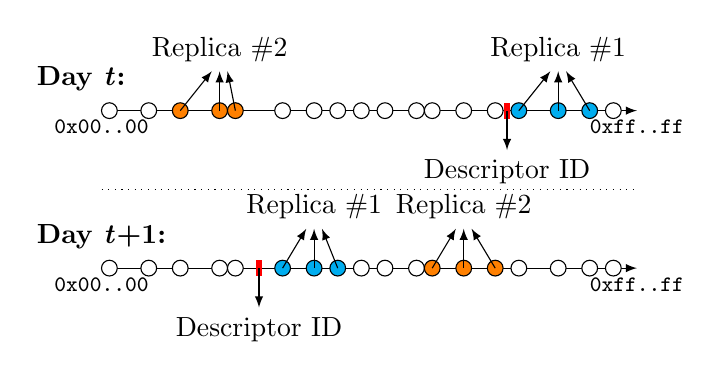
\begin{tikzpicture}

% Day t+1
\node at (0,0.4) {\textbf{Day \emph{t}+1:}};

\draw[,->] (0,0) node[anchor=north] {{\footnotesize \texttt{0x00..00}}} --
	(6.8,0) node[anchor=north] {{\footnotesize \texttt{0xff..ff}}};

\draw[fill=white] (0.1,0) circle (1mm);
\draw[fill=white] (0.6,0) circle (1mm);
\draw[fill=white] (1.0,0) circle (1mm);
\draw[fill=white] (1.5,0) circle (1mm);
\draw[fill=white] (1.7,0) circle (1mm);

\draw[line width=0.7mm, red] (2,-0.1) -- (2,0.1);
\draw[,->] (2,0) -- (2,-0.5) node[anchor=north] {Descriptor ID};

\draw[fill=cyan] (2.3,0) circle (1mm);
\draw[fill=cyan] (2.7,0) circle (1mm);
\draw[fill=cyan] (3.0,0) circle (1mm);
\draw[,->] (2.3,0) -- (2.6,0.5);
\draw[,->] (2.7,0) -- (2.7,0.5) node[anchor=south] {Replica \#1};
\draw[,->] (3.0,0) -- (2.8,0.5);

\draw[fill=white] (3.3,0) circle (1mm);
\draw[fill=white] (3.6,0) circle (1mm);
\draw[fill=white] (4.0,0) circle (1mm);

\draw[fill=orange] (4.2,0) circle (1mm);
\draw[fill=orange] (4.6,0) circle (1mm);
\draw[fill=orange] (5.0,0) circle (1mm);
\draw[,->] (4.2,0) -- (4.5,0.5);
\draw[,->] (4.6,0) -- (4.6,0.5) node[anchor=south] {Replica \#2};
\draw[,->] (5.0,0) -- (4.7,0.5);

\draw[fill=white] (5.3,0) circle (1mm);
\draw[fill=white] (5.8,0) circle (1mm);
\draw[fill=white] (6.2,0) circle (1mm);
\draw[fill=white] (6.5,0) circle (1mm);

\draw[dotted] (0,1.0) -- (6.8,1.0);

% Day t
\node at (0,2.4) {\textbf{Day \emph{t}:\phantom{+1}}};

\draw[,->] (0,2) node[anchor=north] {{\footnotesize \texttt{0x00..00}}} --
(6.8,2) node[anchor=north] {{\footnotesize \texttt{0xff..ff}}};

\draw[fill=white] (0.1,2) circle (1mm);
\draw[fill=white] (0.6,2) circle (1mm);

\draw[fill=orange] (1.0,2) circle (1mm);
\draw[fill=orange] (1.5,2) circle (1mm);
\draw[fill=orange] (1.7,2) circle (1mm);
\draw[,->] (1.0,2) -- (1.4,2.5);
\draw[,->] (1.5,2) -- (1.5,2.5) node[anchor=south] {Replica \#2};
\draw[,->] (1.7,2) -- (1.6,2.5);

\draw[fill=white] (2.3,2) circle (1mm);
\draw[fill=white] (2.7,2) circle (1mm);
\draw[fill=white] (3.0,2) circle (1mm);
\draw[fill=white] (3.3,2) circle (1mm);
\draw[fill=white] (3.6,2) circle (1mm);
\draw[fill=white] (4.0,2) circle (1mm);
\draw[fill=white] (4.2,2) circle (1mm);
\draw[fill=white] (4.6,2) circle (1mm);
\draw[fill=white] (5.0,2) circle (1mm);

\draw[line width=0.7mm, red] (5.15,1.9) -- (5.15,2.1);
\draw[,->] (5.15,2) -- (5.15,1.5) node[anchor=north] {Descriptor ID};

\draw[fill=cyan] (5.3,2) circle (1mm);
\draw[fill=cyan] (5.8,2) circle (1mm);
\draw[fill=cyan] (6.2,2) circle (1mm);
\draw[,->] (5.3,2) -- (5.7,2.5);
\draw[,->] (5.8,2) -- (5.8,2.5) node[anchor=south] {Replica \#1};
\draw[,->] (6.2,2) -- (5.9,2.5);

\draw[fill=white] (6.5,2) circle (1mm);

\end{tikzpicture}
\caption{Each day, an onion service places its descriptor ID at a pseudorandom
	location in Tor's ``hash ring,'' which consists of all HSDir relays
	(illustrated as circles).}
\label{fig:hash-ring}
\end{figure}

\textit{Secret-id-part} depends on three variables: \textit{time-period}
represents the number of days since the Unix epoch; \textit{descriptor-cookie}
is typically unused and hence empty; and \textit{replica} is set to both the
values 0 and 1, resulting in two hashes for \textit{secret-id-part}.  The
concatenation of both \textit{permanent-id} (the onion service's hashed public
key) and \textit{secret-id-part} is hashed, resulting in \textit{descriptor-id},
which determines the position in the DHT.  When arranging all HSDirs by their
fingerprint in ascending order, the three immediate HSDir neighbors in the positive
direction constitute the first replica while the second replica is at another,
pseudorandom location, as shown in Figure~\ref{fig:hash-ring}.  The onion
service's descriptor ID and hence its two replicas changes every day when
\textit{time-period} increments.
